
\section{Sistemi interconnessi - esteso}
È possibile suddividere un sistema comunque complesso, composto da più
sottosistemi che interagiscono tra loro.
Al fine di formalizzare correttamente i sistema interconnessi si presentano i
tre blocchi principali.

Il primo è il blocco sistema, rappresenta il modello di un sistema, disegnato
mediante un rettangolo, con le frecce in ingresso e in uscita si indicano le
variabili di ingresso e uscita.
$$
Y_f(s) = W(s)U(s)
$$
\begin{figure}[h]
\centering
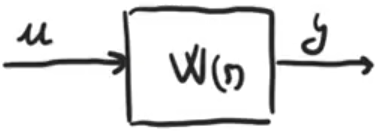
\includegraphics[width=0.3\linewidth]{blocco_sistema}
\end{figure}

Il secondo elemento è il nodo diramatore, ha un ingresso, poi con un punto
calcato si suddividono le uscite (nel dominio del tempo o di Laplace
$$
y_1(t) = y_2(t) = y_3(t) = u(t)
$$
\begin{figure}[h]
\centering
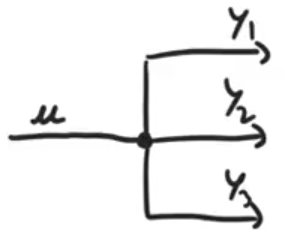
\includegraphics[width=0.3\linewidth]{blocco_nodo}
\end{figure}

\newpage
Il nodo sommatore invece, rappresentato mediante un cerchio o un quadrato
esegue somme o sottrazioni degli ingressi, fornendo una sola uscita
$$
y(t) = u_1(t) - u_2(t) + u_3(t)
$$
\begin{figure}[h]
 \centering
 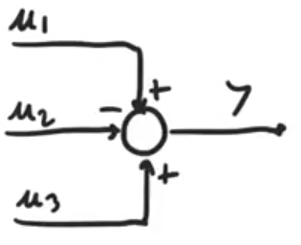
\includegraphics[width=0.3\linewidth]{blocco_sommatore}
\end{figure}
